\subsection{Ecuación Diferencial}

\mode<article>

Nos concentraremos en las ecuaciones diferenciales de la forma

\mode*
\begin{frame}
  \frametitle<presentation>{Ecuación Diferencial}
\begin{equation}\label{EqnEDO}
  y'- f(x, y) = 0
\end{equation}
\end{frame}
\mode<all>
\mode<article>
\noindent lo que nos dice que la derivada de la funicón depende tanto del valor de la misma función
$y$ como de la variable independiente $x$.

Para resolver esta ecuación en forma numérica, debemos discretizar la derivada, 
%
\mode*
\begin{frame}[label=FrameDiferenciasFinitas]
  \frametitle<presentation>{Método de diferencias finitas}
\begin{equation}\label{EqnDeltayDeltax}
    y' = \dfrac{y_{i+1} - y_i}{x_{i+1} - x_i} = \dfrac{y_{i+1} - y_i}{\Delta x}
\end{equation}
\end{frame}

\mode<all>
\mode<article>


\subsubsection{Problemas de condición inicial}

La \autoref{EqnDeltayDeltax}  hace evidente la naturaleza iterativa de la solución numérica. 
Necesitamos una condición inicial, es decir el valor de la función $y$ para algún valor $x_0$ 
que luego propagaremos a todos los valores posibles de $x$ con algúm método adecuado.

\mode*
\begin{frame}[label=FrameCondicionInicial]
  \frametitle<presentation>{CondicionInicial}
\begin{equation}\label{EqnCondicionInicail}
  y_0 = y(x_0)
\end{equation}
\end{frame}
\mode<all>
\mode<article>
Este tipo de razonamiento generalmente se aplica cuando la variable independiente es el tiempo, 
y la condición inicial se \emph{propaga} utilizando la \autoref{EqnDeltayDeltax}
teniendo en cuenta un \emph{paso} $\Delta x$. 
Podemos pensar que en cada paso aproximamos la función por su expansión de Taylor truncada al primer
término. 

\mode*
\begin{frame}<presentation:2|article:1>[label=FrameIteraciones]
  \frametitle<presentation>{Naturaleza Iterativa del método}
  \onslide<1->
  \begin{minipage}{0.4\textwidth}
    \begin{equation}\label{EqnItera}
      \begin{aligned}
	y_1 &= y_0 + y'_0 \Delta x\\
	y_2 &= y_1 + y'_1 \Delta x\\
	\vdots \\
	y_{i+1} &= y_i + y'_i \Delta x
	\vdots \\
      \end{aligned}
    \end{equation}
  \end{minipage}
  \onslide<2>
  \begin{minipage}{0.4\textwidth}
    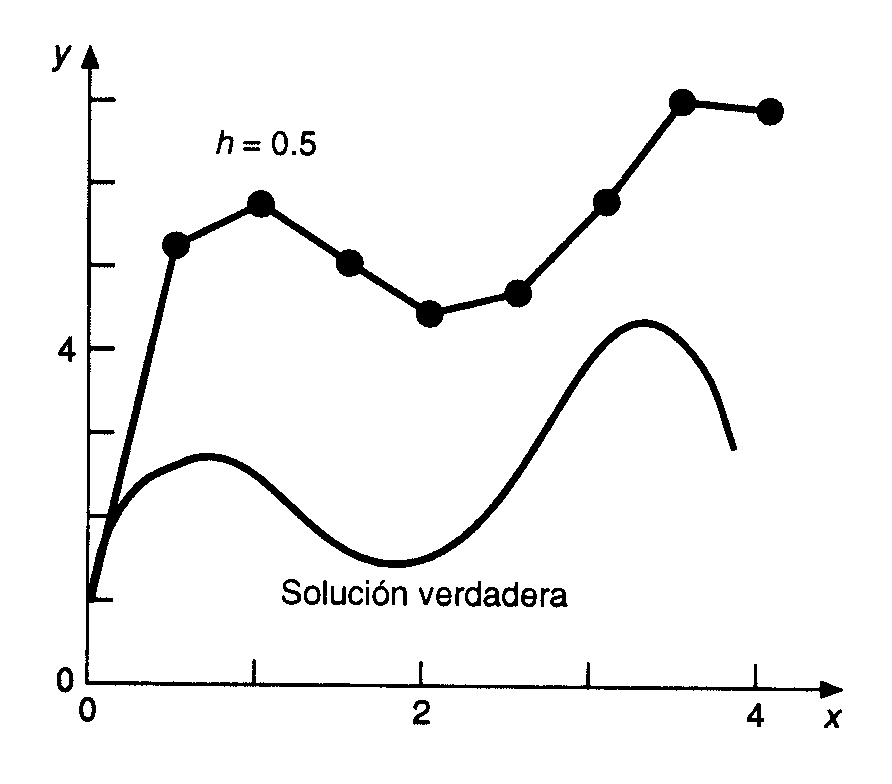
\includegraphics[width=\textwidth]{libreoffice/propagacion.png}
  \end{minipage}

\end{frame}
\mode<all>
\mode<article>

Notemos que la bondad de la aproximación $y_{i+1}$ depende de la aproximación a la derivada de la 
función $y'_i$. En principio la \autoref{EqnEDO} nos da una estimación de dicha derivada, y la 
usaremos para construir nuestros métodos de solución. 

\subsection{Método de Euler}

En este método aproximamos a la función en $x_{i+1}$ por su recta tangente en $x_{i}$. 

\mode*

\begin{frame}<presentation:2|article:1>[label=FrameMetodoEuler]
  \frametitle<presentation>{Método de Euler}
  \center
  \onslide<1->
  \begin{minipage}{0.4\textwidth}
  \begin{equation}
    y_{i+1} = y_i + f(x_i, y_i ) \Delta x
  \end{equation}
  \end{minipage}
  \onslide<2>
  \begin{minipage}{0.4\textwidth}
    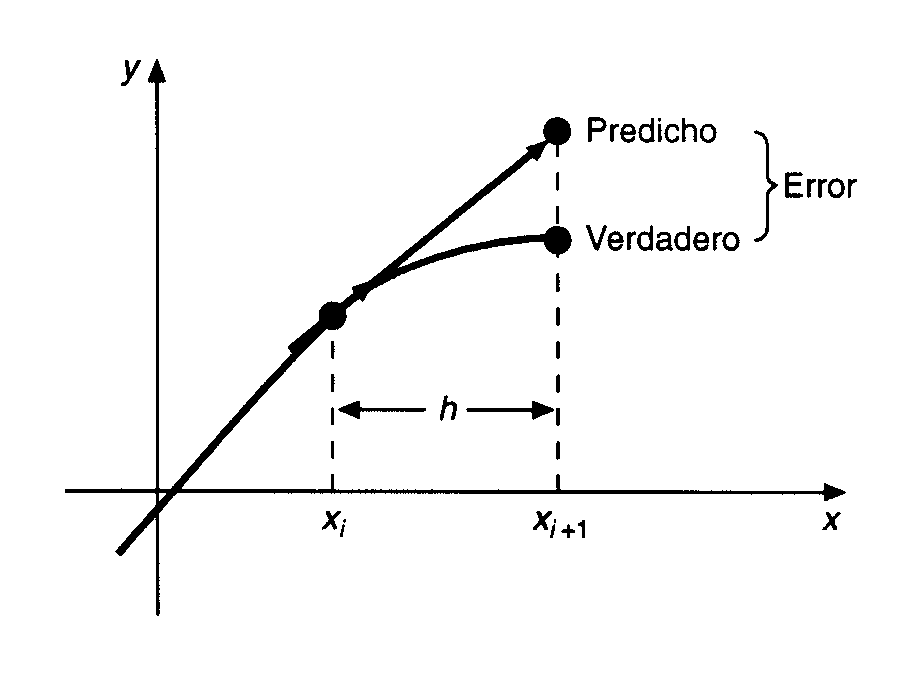
\includegraphics[width=\textwidth]{libreoffice/prediccion_Euler.png}
  \end{minipage}
\end{frame}
\mode<all>

\mode<article>

\subsection{Método de Runge-Kutta}

Para este método, se aproxima la función por su expansión de Taylor pero se
realizan correcciones sucesivas a la derivada de manera que necesitamos definir
cuatro constantes, que de penden de las anteriores, hasta poder aproximar la
derivada. 
\mode*
\begin{frame}<presentation:2|article:1>[label=FrameMethodRungeKutta]
  \frametitle<presentation>{Método de Runge Kutta de orden 4}
  \center
  \onslide<1->
  \begin{minipage}{0.4\textwidth}
    \begin{equation}
      \begin{aligned}
	k_1 &= f(x_i, y_i)\\
	k_2 &= f \Big( x_i + \frac{1}{2} \Delta x, y_i + \frac{1}{2} k_1 \Delta x \Big)\\
	k_3 &= f \Big( x_i + \frac{1}{2} \Delta x, y_i + \frac{1}{2} k_2 \Delta x \Big)\\
	k_4 &= f \Big( x_i \Delta x, y_i + k_3 \Delta x \Big)\\
	y_{i+1} &= y_i+\frac{1}{6} \Big( k_1 + 2 k_2 + 2 k_3 + k_4 \Big) \Delta x
      \end{aligned}
    \end{equation}
  \end{minipage}
  \onslide<2>
  \begin{minipage}{0.4\textwidth}
    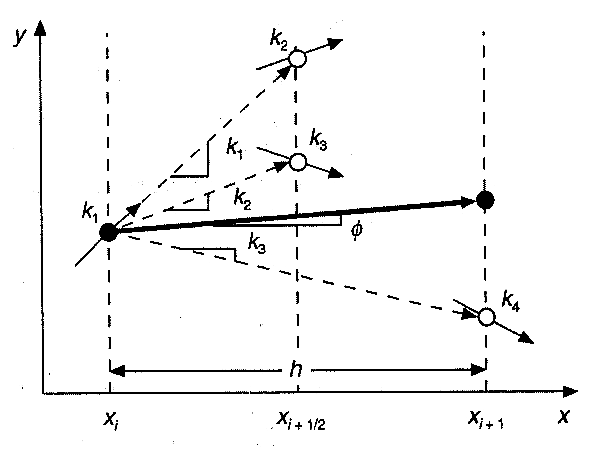
\includegraphics[width=\textwidth]{libreoffice/propagacion-RungeKutta.png}
  \end{minipage}
\end{frame}
\mode<all>
\mode<article>

\subsection{Ecuaciones de orden superior}

Estos métodos de propagación se aplican directamente a ecuaciones de orden 1,
puesto que dependen de aproximar la primer derivada de la función incógnita. 
Podemos extenderlo fácilmente a ecuaciones de orden superior de la siguiente manera.
Supongamos una ecuación de orden 2, 
\mode*
\begin{frame}[label=FrameEcuacionOrden2]
  \frametitle<presentation>{Ecuación de Orden dos}
  \begin{equation}
    y'' + \eta y' + f(x, y) = 0
  \end{equation}
\end{frame}
\mode<all>
\mode<article>

Vamos a operar tomando un cambio de variables sencillo para definir una nueva variable vectorial 
incógnita, 
\mode*
\begin{frame}[label=FrameVariableVectorial]
  \frametitle<presentation>{Nueva Variable Vectorial}
  \begin{equation}
    \begin{aligned}
      X &= y &\text{ (función ) } \\
      Y &= y' &\text{(derivada) }\\
      \mathbf{V} &= \begin{pmatrix} X \\ Y  \end{pmatrix} \\
	\mathbf{V'} &=  \begin{pmatrix} X \\ Y  \end{pmatrix}' &= 
	  \begin{pmatrix}   Y \\ -\eta Y - f(x, y)  \end{pmatrix}
    \end{aligned}
  \end{equation}
\end{frame}
\mode<all>
\mode<article>

Con lo cual tenemos definido una nueva ecuación vectoria, donde hemos reemplazado 
la función incógnita por un vector cuyas componentes son la función y su primera 
derivada. Hemos reemplazado también la función característica de la ecuación por una
función también vectorial, 

\mode*
\begin{frame}[label=FrameEcuacionOrdenSuparior]
  \frametitle<presentation>{Nueva Ecuacion de orden 1}
  \begin{equation}
    \mathbf{F}(x, X, Y) = \begin{pmatrix} Y\\ \eta Y - f(x, X)   \end{pmatrix}
  \end{equation}
\end{frame}
\mode<all>
\mode<article>

Resulta entonces que podemos aplicar los mismos métodos para resolver la variable
$\mathbf{V}$. Por ejemplo para el método de Euler, 
\mode*
\begin{frame}[label=FrameEulerVectorial]
  \frametitle<presentation>{Euler Vectorial}
  \begin{equation}\label{EqnEulerVec}
    \begin{aligned}
      \mathbf{V_i} &= \begin{pmatrix} X_{i-1} \\ Y_{i-1} \end{pmatrix} + 
	\Delta x F\Big( x_{i-1}, X_{i-1}, Y_{i-1} \Big) \\
	{} &= 
	\begin{pmatrix} 
	  X_{i-1} + \Delta x Y_{i-1} \\ 
	  Y_{i-1} + \Delta x \Big( \eta Y_{i-1} - f(x_{i-1} , X_{i-1}\Big)
	\end{pmatrix}
    \end{aligned}
  \end{equation}
\end{frame}
\mode<all>
\mode<article>

vemos que basta identificar la función $F(x, X, Y)$ para poder aplicar cualquiera de los métodos vistos.

\mode*

\mode<all>
